\chapter{Solução}

A solução proposta por este trabalho foi implementada em cima do controlador
POX \citep{pox}. 
Uma abstração da rede em forma de grafo foi construída como um módulo 
do controlador da rede.
Esse grafo, em tempo real, representando a rede é a base para toda computação
executada sobre a rede.
A solução objetiva simplificar o gerenciamento em redes reduzindo o volume 
de computações ao longo dos nós da rede aproveitando a separação do plano 
de dados e do plano de controle.

\section{A abstração em grafos}

O grafo propost é representado por $G=(V, A)$, em que $V$ e $A$ são conjuntos
finitos de vértices e arestas, respectivamente.
Cada vértice $v \in V$ representa um computador (\emph{host}) ou comutador
(\emph{switch}) dentro da rede.
Cada aresta $u \to v \in A$ representa um enlace (\emph{link}) entre dois
vértices.
O peso das arestas $g(u, v)$ descreve a quantidade de \emph{bytes} trafegados
na aresta entre os dois vértices.

\section{Controlador}
\label{sec:controller}

O controlador POX é um arcabouço para elaboração de módulos/programas 
em Redes Definidas por \emph{Software}.
Totalmente voltado para pesquisa, o POX é um controlador simples, 
escrito na linguagem de programação \emph{Python}.

Ao ser carregado, o POX, executa o seu núcleo (\emph{core}). 
Esse módulo principal, é responsável por carregar os demais 
módulo e garantir a comunição entre eles.
Ele exporta uma interface baseada em eventos. 
Eventos que descrevem ou representam ações ocorridas na rede.
Um módulo implementado dentro do controlador POX pode ser um 
produtor/consumidor de eventos.

O POX contém alguns módulos de descoberta que publicam eventos relacionados
à topologia da rede:

\begin{itemize}

\item{\emph{topology}}: 

O módulo \emph{topology}, é responsável por mapear a topologia da rede. 
Utilizando os recursos do \emph{core}, ele atua como um canal de eventos 
relacionados à topologia e que os demais módulos podem fazer escuta 
(\emph{listening}).

\item{\emph{host\_tracker}}: 

Seu objetivo é buscar e rastrear informações sobre os computadores 
(\emph{hosts}) dentro da rede.

\item{\emph{openflow.topology}}: 

Um controle de topologia específico para switches OpenFlow.
Ele é integrado com o módulo \emph{topology} do POX.

\item{\emph{openflow.discovery}}: 

Identifica links entre switches OpenFlow por meio do protocolo LLDP.

\item{\emph{misc.dhcpd}}:

Servidor de DHCP para configuração dinâmica da rede IP.

\end{itemize}

Esses módulos são os módulos relevantes para o presente trabalho.
Existem diversos outros módulos dentro do controlador POX, no entanto
eles não serão abordados nesse trabalho.

\section{Projeto de implementação}

A proposta do módulo em grafos é integrada aos módulos citados na seção do 
\ref{sec:controller} (Controlador).
A implementação do módulo é composta por cinco classes:

\begin{itemize}
    \item{Graph}: 
        
        Classe responsável por gerenciar o grafo.
        Todo o tratamento de eventos é feito por essa classe.
        O controle de criação, remoção e atualização de vertices e arestas 
        é feito por essa classe.
    \item{GraphEntity}: 
        
        Classe abstrata que implementa arestas e vértices.
        Essas entidades, vértices e arestas, herdam da classe 
        \emph{GraphEntity}
    \item{Vertex}: 
        
        Classe que representa os vértices do grafo.
        Vértices podem ser máquinas (\emph{hosts}) ou comutadores
        (\emph{switches})
    \item{Edges}: 
        
        Classe que representa as arestas do grafo.
        Arestas são enlaces (\emph{links}) entre dois vértices.
        O peso das arestas é um atributo dos objetos dessa classe.
    \item{GraphManager}: 
        
        Classe responsável por executar computações no grafo.
        Toda implementação de algoritmos em grafos é feita dentro dessa classe.
\end{itemize}

\section{Vértices}

O módulo \emph{topology} dispara os eventos \emph{HostJoin}, \emph{HostLeave},
\emph{SwitchJoin}, \emph{SwitchLeave}.
Ao ser carregado, o módulo \emph{graph} passa a escutar esses eventos.
Quando eles são disparados pelo \emph{topology} o grafo é atualizado.
Assim, os vértices são criados no grafo em tempo real, à medida que os
eventos ocorrem na rede.

Todo vértice tem um identificador único.
No caso de vértices do tipo computador (\emph{Host}), o identificador 
é o endereço MAC (\emph{Media Access Control}) da interface de rede.
Já os vértices do tipo comutador (\emph{Switch}) são identificados pelo 
DPID (\emph{Datapath ID}) que é associado ao comutador no momento de sua 
conexão com o controlador.

\section{Arestas}

As arestas podem ser enlaces (\emph{links}) entre computadores e comutadores ou
entre comutadores.
Para a identificação das arestas entre os comutadores, o módulo \emph{graph} 
escuta o evento \emph{LinkJoin} que é disparado pelo módulo 
\emph{openflow.discovery}.
Os enlaces entre computadores e comutadores é identificado quando, ao 
adicionar um vértice do tipo \emph{Host}, esse vértice possuir a informação
de qual comutador ele está diretamente conectado.

O peso das arestas é obtido através da leitura dos contadores de fluxos 
presentes nos comutadores OpenFlow.
Para o módulo \emph{graph} são lidos os contadores de fluxo da porta 
no switch. 
A lista de contadores é apresentada na Tabela \ref{tbl:counters} e em 
\citep{ofprotocol2015}.
Através da contagem desses fluxos é possível mensurar o tráfego 
decorrente na aresta.


\begin{table}[h!]
    \centering
    \begin{tabular}{| l | l |}
    \hline
    \textbf{Contador} & \textbf{Bits} \\ \hline
    Pacotes Recebidos & 64 \\ \hline
    Pacotes Transmitidos & 64 \\ \hline
    Bytes Recebidos & 64 \\ \hline
    Bytes Transmitidos & 64 \\ \hline
    Drops Recebidos & 64 \\ \hline
    Drops Transmitidos & 64 \\ \hline
    Erros Recebidos & 64 \\ \hline
    Erros Transmitidos & 64 \\ \hline
    Erros de Frames Recebidos & 64 \\ \hline
    Erros de Transbordo Transmitidos & 64 \\ \hline
    Erros de CRC Recebidos & 64 \\ \hline
    Colisões & 64 \\
    \hline
    \end{tabular}
    \caption{Contadores de fluxos por Porta}
    \label{tbl:counters}
\end{table}


\section{O módulo \emph{host\_tracker}}

Além da criação do módulo composto pelas classes acima descritas, alterações
no módulo \emph{host\_tracker} foram feitas.
O \emph{host\_tracker} identifica os pacotes de DHCP (\emph{Dinamic Host
Configuration Protocol}) e descobre novos computadores (\emph{hosts}) na rede.
Ao construir um novo objeto da classe \emph{Host} o \emph{topology} dispara
um evento de \emph{HostJoin} ao qual o módulo \emph{graph} irá atualizar
o grafo da rede.

Assim como \emph{openflow.discovery} identifica os comutadores, o 
\emph{host\_tracker} o faz para máquinas (\emph{hosts}).
Isso é feito através de um interceptador ARP (\emph{Address Resolution 
Protocol}).
Todos os comutadores (\emph{switches}) OpenFlow são programados para encaminhar
os pacotes de consulta \emph{ARPQuery} para o controlador.
Se essa consulta for destinada a um computador conhecido pelo
\emph{host\_tracker}, um pacote de resposta \emph{ARPReply} é contruído e 
encaminhado para a máquina que originou a consulta.

Periodicamente, o \emph{host\_tracker} envia mensagens \emph{ARPQuery} falsas
para todos os computadores conhecidos a fim de verificar se eles estão ativos
na rede.
Através dos contadores dos comutadores OpenFlow, o \emph{host\_tracker} 
monitora a atividade nos enlaces podendo inferir a presença de atividade
dos computadores sem ter que enviar mensagens ARP.

\section{Interface de programação}

O módulo \emph{Graph} exporta uma interface de programação (API).
Através dessa interface, outros módulos do controlador podem requisitar 
informações da topologia, do tráfego e do estado da rede através do grafo.
Essas informações podem ser utilizadas para implementar serviços em diversas
camadas de rede que necessitam dessa informação.
Os metodos permitidos por esse módulo são:

\begin{itemize}
    \item \emph{get\_vertex(id)}

        Retorna um vértice do grafo (máquinas ou comutadores). 
        O parâmetro \emph{id} pode ser um endereço MAC ou o DPID.

    \item \emph{get\_adjacents(id)}

        Dado um vértice, retorna sua lista de adjacência.

    \item \emph{snapshot()}

        Retorna o estado instantâneo da aplicação na forma de duas coleções,
        uma de vértices e outra de arestas.
\end{itemize}

\section{Integração}

A integração do módulo \emph{graph} com os demais módulos do controlador POX
é apresentado na figura \ref{fig:graph-integration}.
A forma como o controlador POX implementa seu controle de eventos é 
inteiramente dependente do seu núcleo (\emph{core}).
O núcleo é responsável por notificar os módulos inscritos (que fazem escuta) 
nos eventos a serem disparados.
Toda troca de mensagens passa primeiramente por ele.
A implementação do módulo \emph{graph} está disponível em 
\url{https://github.com/pantuza/pox}.

Os módulos \emph{openflow.discovery} e \emph{openflow.topology} identificam 
comutadores (\emph{switches}) e notificam o módulo \emph{topology} através do
\emph{core}. 
O \emph{topology} por sua vez, cria o evento que causa a atualização no grafo
através do módulo \emph{graph}.

As ações referentes a computadores são de responsabilidade dos módulos
\emph{misc.dhcp} e \emph{host\_tracker}.
Nesses casos, o \emph{topology} também é comunicado atraveś do \emph{core} e
dispara eventos que atualizam o grafo através do módulo \emph{graph}.

Caso algum módulo queira recuperar informações topológicas ou do estado da
rede, ele o faz através de chamadas à interface (API) do módulo \emph{graph}.

\begin{figure}[h!]
    \centering
    \label{fig:graph-integration}
    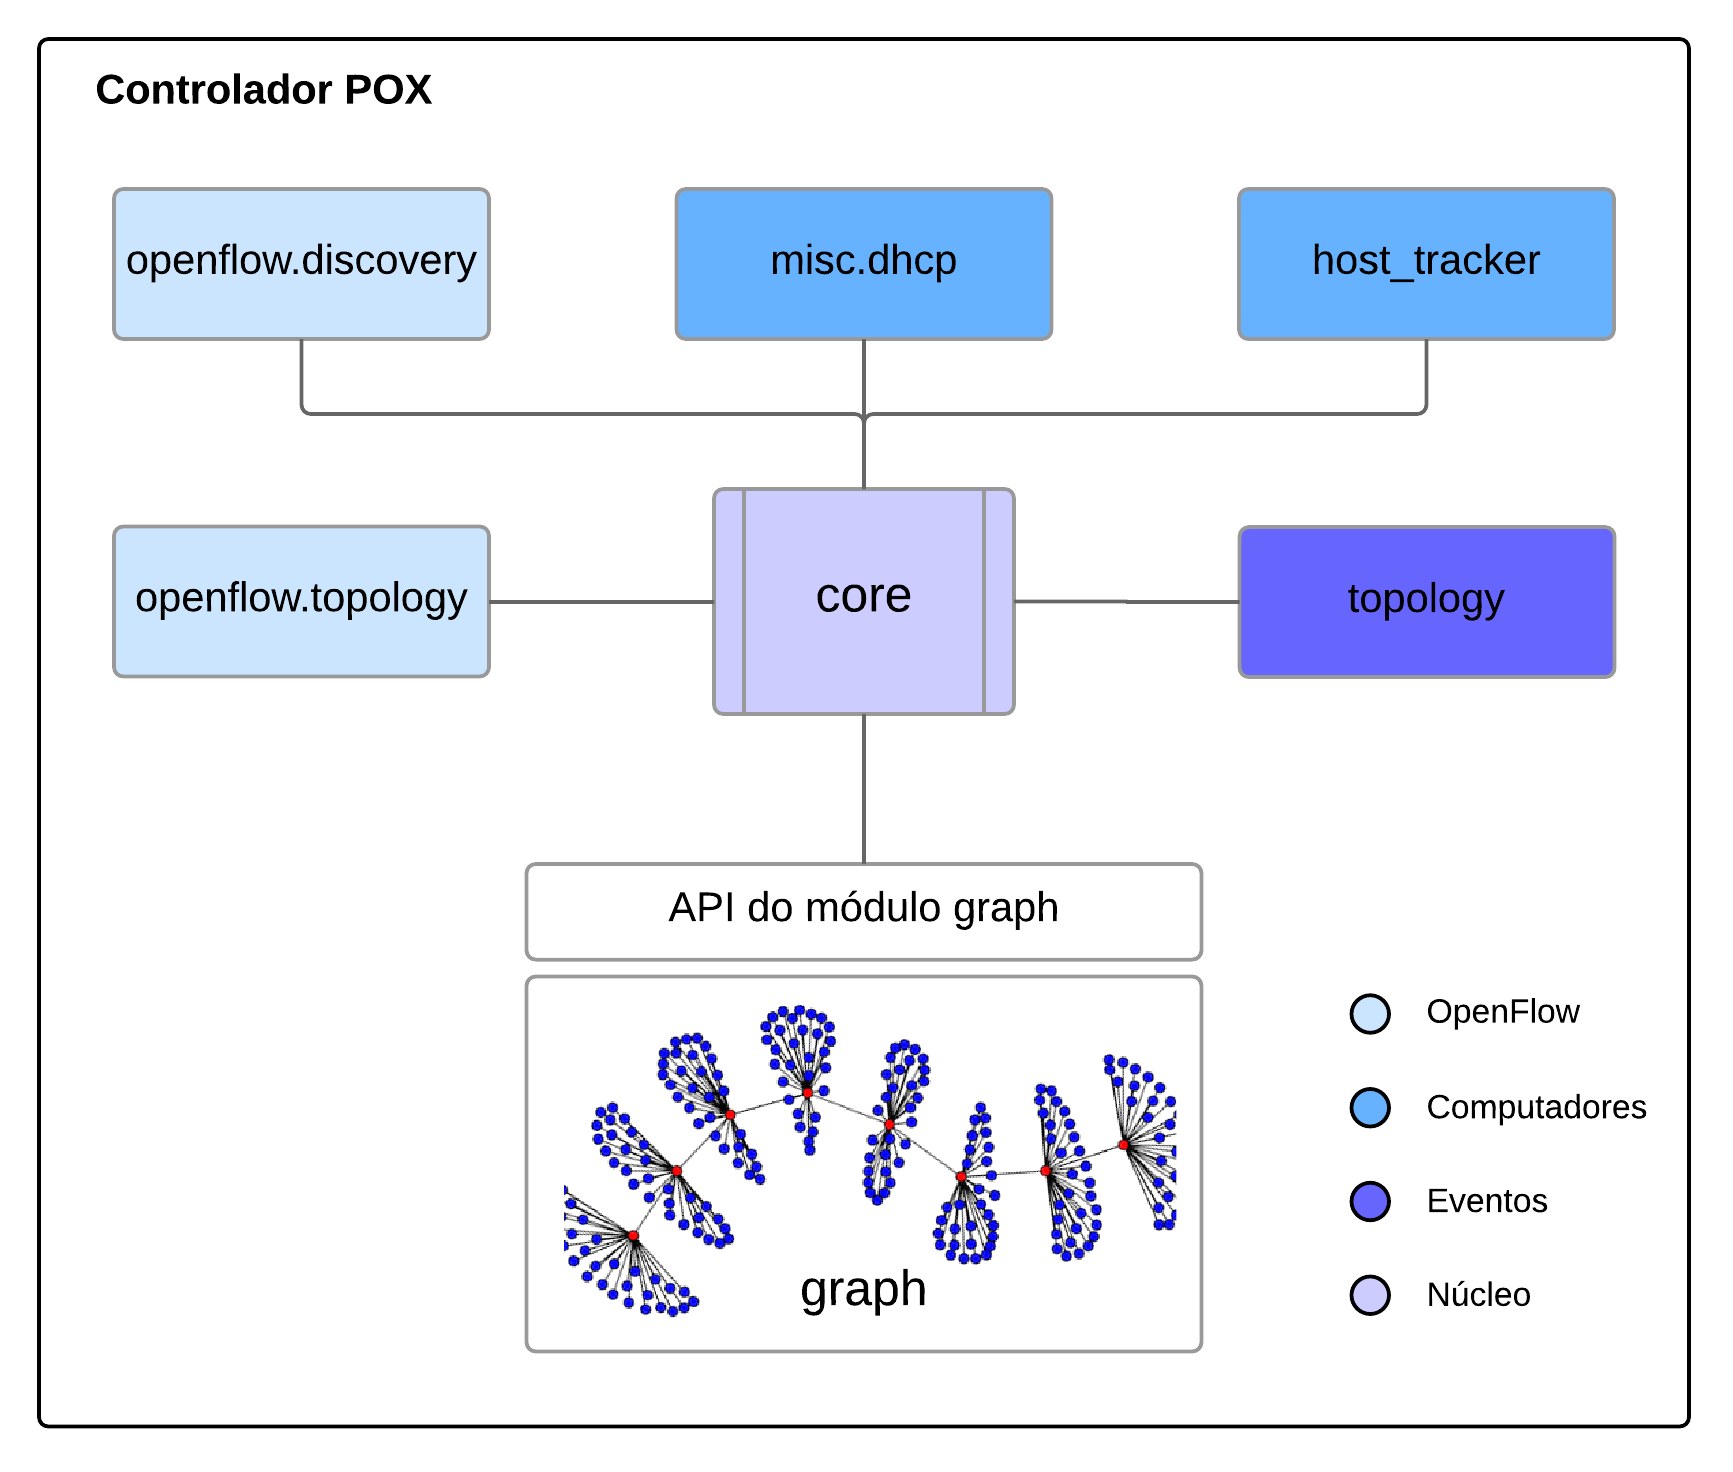
\includegraphics{img/graph-module-integration}
    \caption{Integração do módulo \emph{graph} no controlador POX}
\end{figure}

